\documentclass[tikz,border=8pt]{standalone}
% Shared look for every TikZ diagram. Load with % Shared look for every TikZ diagram. Load with % Shared look for every TikZ diagram. Load with \input{../../tools/tikz-style.tex}
\usepackage[T1]{fontenc}
\usepackage{lmodern}
\renewcommand{\sfdefault}{lmr}  % diagrams use the same serif as the text
\usetikzlibrary{arrows.meta, positioning, shapes.geometric, calc, fit, backgrounds}
\definecolor{cblue}{HTML}{4C78A8}
\definecolor{corange}{HTML}{F58518}
\definecolor{cgreen}{HTML}{54A24B}
\definecolor{cred}{HTML}{E45756}
\definecolor{cpurple}{HTML}{B279A2}
\definecolor{cgrey}{HTML}{6B6B6B}
\tikzset{
  every picture/.style={font=\sffamily, line width=1.2pt},
  box/.style={draw=#1, fill=#1!12, rounded corners=4pt, align=center, inner sep=7pt, minimum height=1.1cm},
  box/.default=cgrey,
  arrow/.style={-{Stealth[length=3mm]}, draw=cgrey, line width=1.4pt},
  title/.style={font=\sffamily\bfseries\Large},
  note/.style={font=\sffamily\small, text=cgrey, align=center},
}
\AtBeginDocument{\hyphenpenalty=10000 \exhyphenpenalty=10000}

\usepackage[T1]{fontenc}
\usepackage{lmodern}
\renewcommand{\sfdefault}{lmr}  % diagrams use the same serif as the text
\usetikzlibrary{arrows.meta, positioning, shapes.geometric, calc, fit, backgrounds}
\definecolor{cblue}{HTML}{4C78A8}
\definecolor{corange}{HTML}{F58518}
\definecolor{cgreen}{HTML}{54A24B}
\definecolor{cred}{HTML}{E45756}
\definecolor{cpurple}{HTML}{B279A2}
\definecolor{cgrey}{HTML}{6B6B6B}
\tikzset{
  every picture/.style={font=\sffamily, line width=1.2pt},
  box/.style={draw=#1, fill=#1!12, rounded corners=4pt, align=center, inner sep=7pt, minimum height=1.1cm},
  box/.default=cgrey,
  arrow/.style={-{Stealth[length=3mm]}, draw=cgrey, line width=1.4pt},
  title/.style={font=\sffamily\bfseries\Large},
  note/.style={font=\sffamily\small, text=cgrey, align=center},
}
\AtBeginDocument{\hyphenpenalty=10000 \exhyphenpenalty=10000}

\usepackage[T1]{fontenc}
\usepackage{lmodern}
\renewcommand{\sfdefault}{lmr}  % diagrams use the same serif as the text
\usetikzlibrary{arrows.meta, positioning, shapes.geometric, calc, fit, backgrounds}
\definecolor{cblue}{HTML}{4C78A8}
\definecolor{corange}{HTML}{F58518}
\definecolor{cgreen}{HTML}{54A24B}
\definecolor{cred}{HTML}{E45756}
\definecolor{cpurple}{HTML}{B279A2}
\definecolor{cgrey}{HTML}{6B6B6B}
\tikzset{
  every picture/.style={font=\sffamily, line width=1.2pt},
  box/.style={draw=#1, fill=#1!12, rounded corners=4pt, align=center, inner sep=7pt, minimum height=1.1cm},
  box/.default=cgrey,
  arrow/.style={-{Stealth[length=3mm]}, draw=cgrey, line width=1.4pt},
  title/.style={font=\sffamily\bfseries\Large},
  note/.style={font=\sffamily\small, text=cgrey, align=center},
}
\AtBeginDocument{\hyphenpenalty=10000 \exhyphenpenalty=10000}

\begin{document}
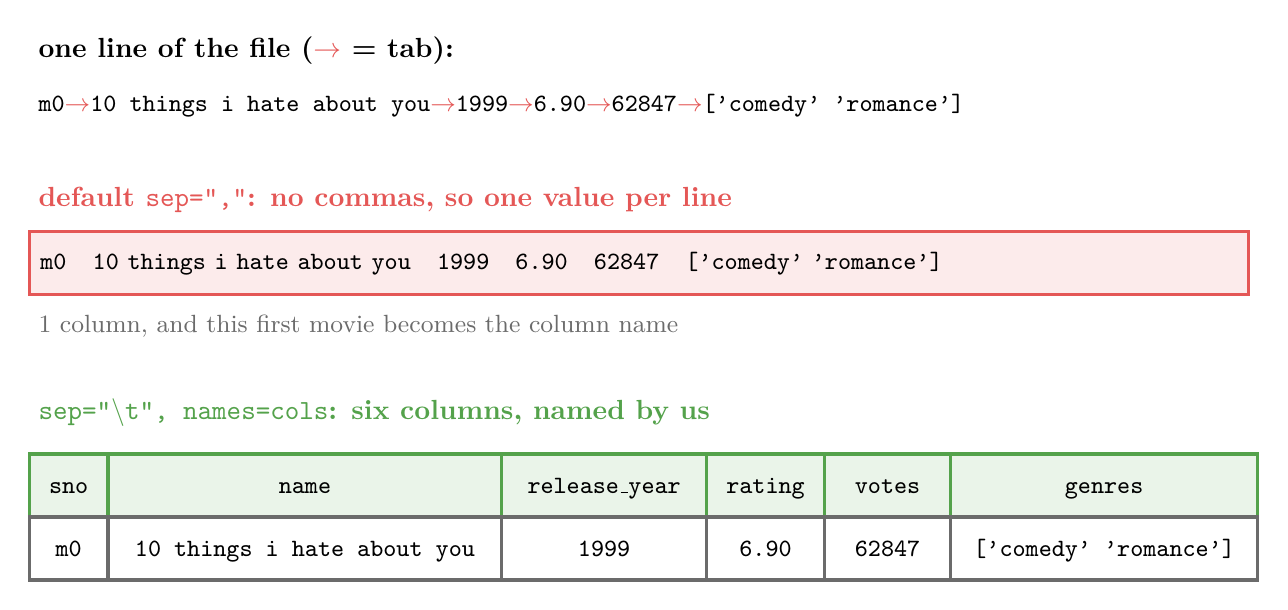
\begin{tikzpicture}[c/.style={draw=#1, fill=#1!12, minimum height=0.8cm, font=\ttfamily\small, inner sep=4pt},
                    tab/.style={font=\sffamily\scriptsize\bfseries, text=cred}]
  \node[anchor=west, font=\sffamily\bfseries] at (0,2.2) {one line of the file (\textcolor{cred}{$\to$} = tab):};
  \node[anchor=west, font=\ttfamily\small] at (0,1.5) {m0\textcolor{cred}{$\to$}10 things i hate about you\textcolor{cred}{$\to$}1999\textcolor{cred}{$\to$}6.90\textcolor{cred}{$\to$}62847\textcolor{cred}{$\to$}['comedy' 'romance']};
  % default
  \node[anchor=west, font=\sffamily\bfseries, text=cred] at (0,0.3) {default \texttt{sep=","}: no commas, so one value per line};
  \node[c=cred, anchor=west, text width=15.2cm] at (0,-0.5) {m0\quad 10 things i hate about you\quad 1999\quad 6.90\quad 62847\quad ['comedy' 'romance']};
  \node[note, anchor=west] at (0,-1.3) {1 column, and this first movie becomes the column name};
  % fixed
  \node[anchor=west, font=\sffamily\bfseries, text=cgreen] at (0,-2.4) {\texttt{sep="\textbackslash t", names=cols}: six columns, named by us};
  \foreach \h/\v/\w/\x in {sno/m0/1.0/0, name/10 things i hate about you/5.0/1.0, release\_year/1999/2.6/6.0,
                           rating/6.90/1.5/8.6, votes/62847/1.6/10.1, genres/{['comedy' 'romance']}/3.9/11.7} {
    \node[c=cgreen, anchor=north west, minimum width=\w cm, text height=1.8ex, text depth=0.5ex, font=\ttfamily\small\bfseries] at (\x,-2.9) {\h};
    \node[c=cgrey, fill=white, anchor=north west, minimum width=\w cm, text height=1.8ex, text depth=0.5ex] at (\x,-3.7) {\v};
  }
\end{tikzpicture}
\end{document}
